\documentclass[12pt,letterpaper]{article}
\usepackage{fullpage}
\usepackage[top=2cm, bottom=4.5cm, left=2.5cm, right=2.5cm]{geometry}
\usepackage{amsmath,amsthm,amsfonts,amssymb,amscd}
\usepackage{lastpage}
\usepackage{enumerate}
\usepackage{fancyhdr}
\usepackage{mathrsfs}
\usepackage{xcolor}
\usepackage{graphicx}
\usepackage{listings}
\usepackage{hyperref}

\hypersetup{%
  colorlinks=true,
  linkcolor=blue,
  linkbordercolor={0 0 1}
}
 
\renewcommand\lstlistingname{Algorithm}
\renewcommand\lstlistlistingname{Algorithms}
\def\lstlistingautorefname{Alg.}

\lstdefinestyle{Python}{
    language        = Python,
    frame           = lines, 
    basicstyle      = \footnotesize,
    keywordstyle    = \color{blue},
    stringstyle     = \color{green},
    commentstyle    = \color{red}\ttfamily
}

\setlength{\parindent}{0.0in}
\setlength{\parskip}{0.05in}
\begin{document}






Foundations of Applied Math\\
 HW \#4
 Due Friday, Oct. 9

\textbf{Reminder} You need to turn in a .zipped folder that contains your .tex file, your image files, your python file and the tex file must compile.
Rename the .tex file: HW4$\_$YourLastName.tex and call the folder which you will compress: HW4$\_$YourLastName

Please make sure you learn the examples in 1.4 before you do this HW.

\begin{enumerate}

\item 1.4) Do \#6b this time using python. For each of the four cases please make sure you generate a plots like the ones we generated in HW 3 using Excel.  (On Friday I will show you how to generate plots using arrays in python and how to generate a legend). Include your python file so that I can run it and paste your 8 graphs here. (Each case should have 2 graphs.)
\begin{enumerate}
  \item Case A: \\ 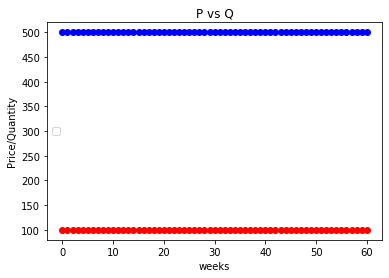
\includegraphics[scale = .5]{1.4 6 a.png}
  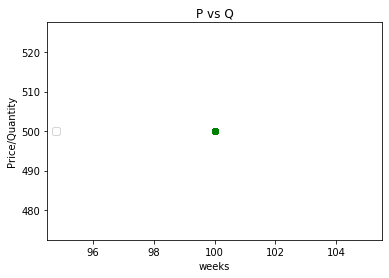
\includegraphics[scale = .5]{1.4 6 a2.png}
  \item Case B: \\ 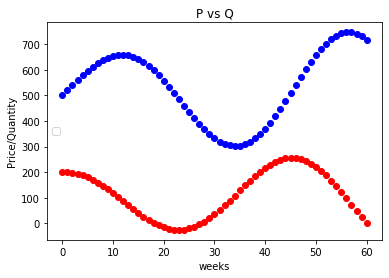
\includegraphics[scale = .5]{1.4 6 b1.png}
  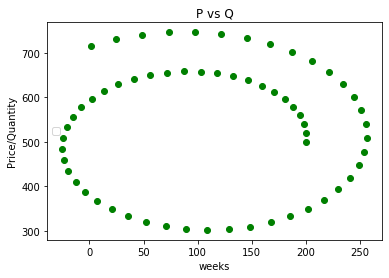
\includegraphics[scale = .5]{1.4 6 b2.png}
  \item Case C: \\ 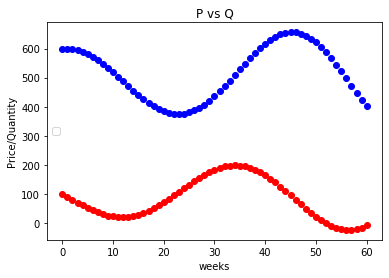
\includegraphics[scale = .5]{1.4 6 c2.png}
  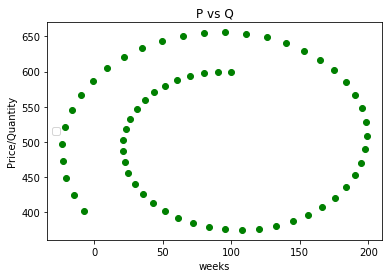
\includegraphics[scale = .5]{1.4 6 c1.png}
  \item Case D: \\ 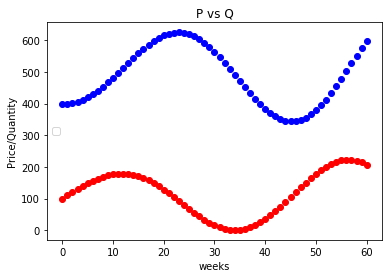
\includegraphics[scale = .5]{1.4 6 d1.png}
  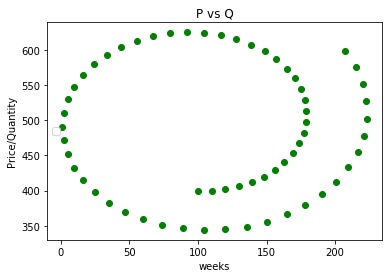
\includegraphics[scale = .5]{1.4 6 d2.png}
\end{enumerate}

\item 1.4) Using arrays plot $\frac{x^2}{25}+\frac{y^2}{9}=1$ using python.  Make sure your plot is one color curve. Have your last two lines be: 

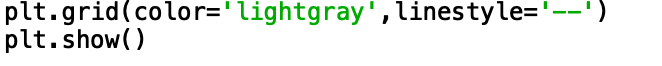
\includegraphics[scale=.75]{lasttwo.png}

Include your python file so that I can run it and paste your graph here. Hint- you will need to solve for $y$.
\\
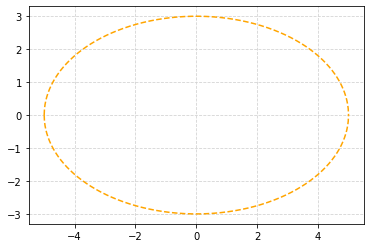
\includegraphics[scale=.75]{number2.png}\\
Python file is inlcuded in the zipped folder. 

\item 
Consider the following  model for two species.   
\begin{eqnarray*}
x_{n+1} &=& 0.8x_{n} + 0.001x_{n}y_{n}\\
y_{n+1}&=& y_{n} +0.0001y_{n}(3000-y_{n}) -0.004x_{n}y_{n}
\end{eqnarray*}

\begin{enumerate}
\item[a)] This model is a predator-prey model. Explain why. Also state which species is the predator. \\
This model shows that the change in $x_{n+1}$ increases depending on how many interactions 
there are between $x$ and $y$. However, $y$ decreases depending on how many interactions there are between 
$x$ and $y$. Therefore, $x$ is the predator and $y$ is the prey. 

\item[b)] According to the model, what happens to the population of the predator if there is no prey present? Support your answer with a graph of predators vs. $n$.\\
The population of the predators will only decrease if there are no prey. Specifically, only 80\%
of the predator population will survive in the next iteration if there are no prey. Looking
at the graph of $n$ vs $p$, we see that the population of the predators do indeed go down: \\
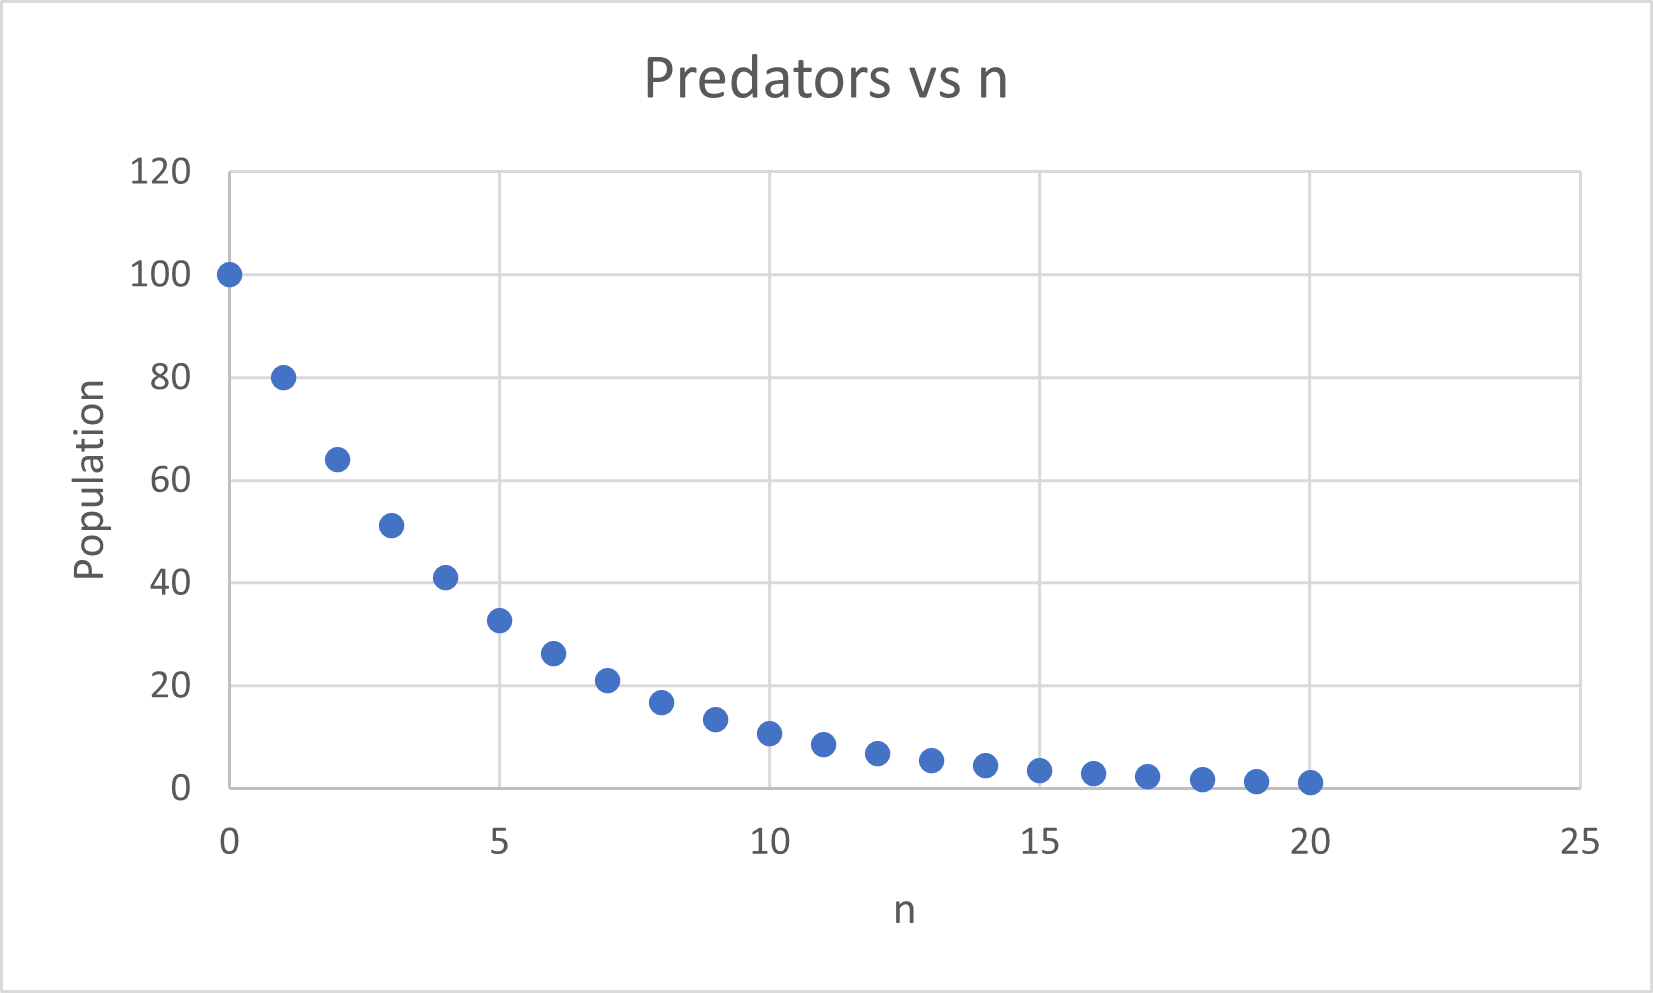
\includegraphics[scale = .5]{n vs p.png} 

Plotting the $\Delta p_{n}$ vs $p$ graph, we also see that the change is indeed $-20\%$ between $p_{n}$ and $p_{n+1}$ or 
80\% of the population. \\
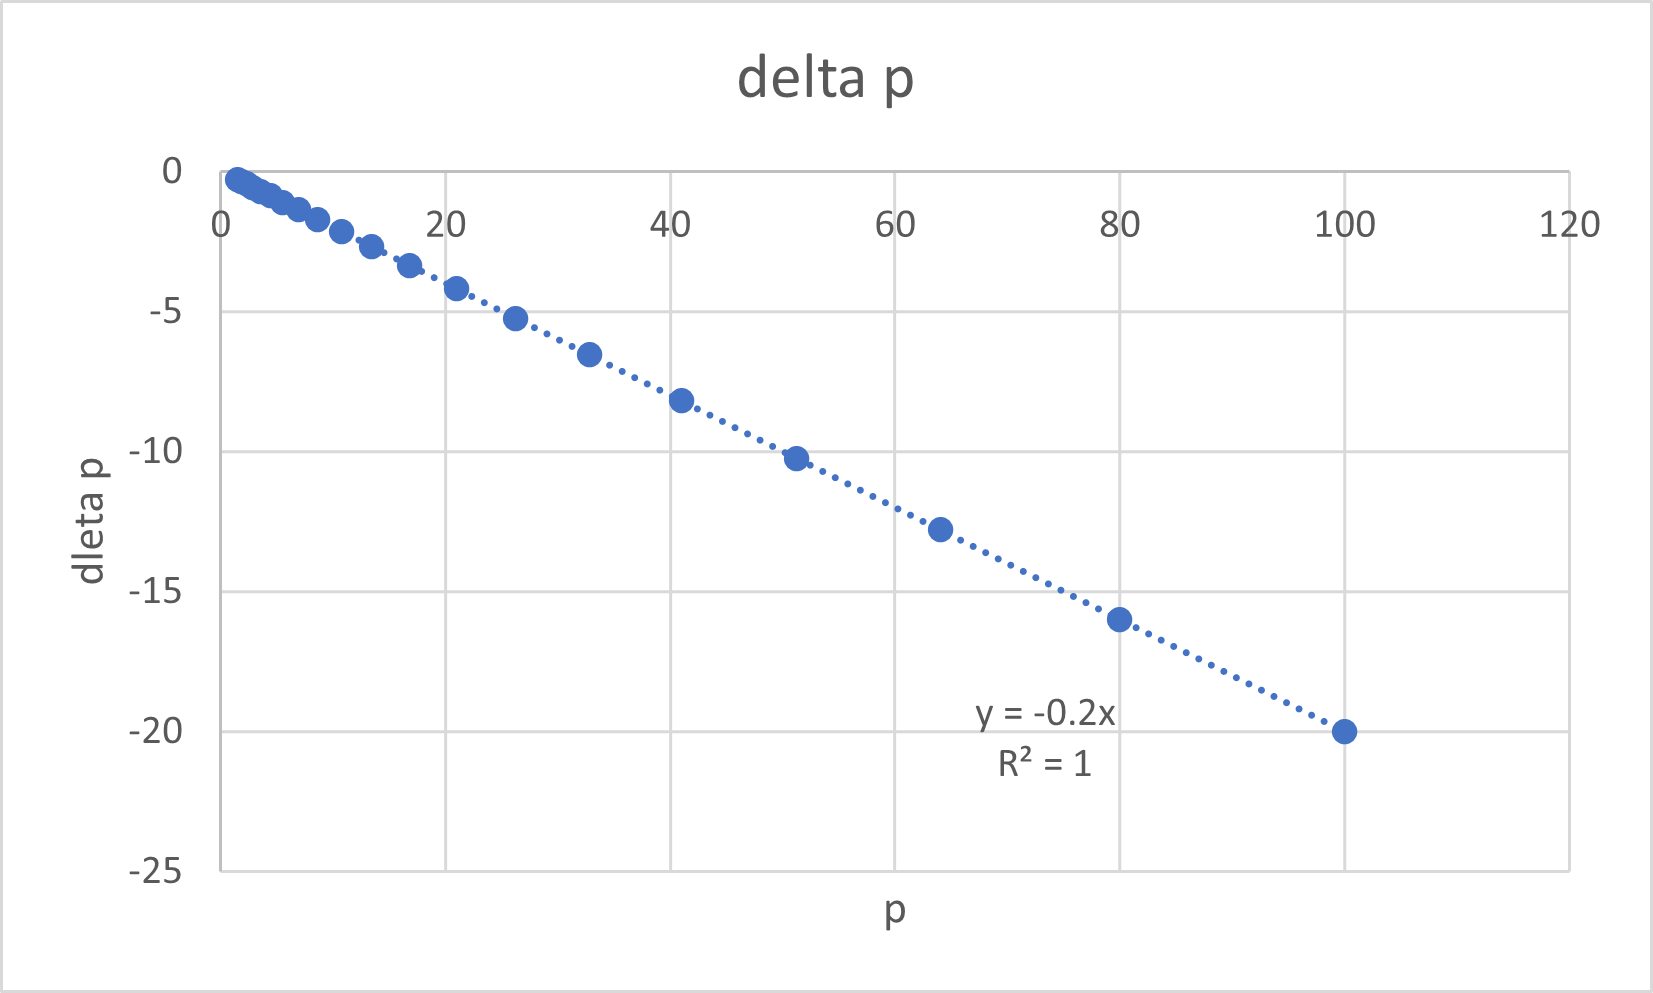
\includegraphics[scale = .5]{delta p vs p.png}

\item[c)] According to the model, will the population of the prey experience unlimited population growth if there are no predators present?\\
The population of the prey will not experience unlimited population growth because of the second 
term. This logistic term will force the maximum population to be 3000. 

\end{enumerate}




\item  2.2, \#3\\
By Hooke's law: 
\begin{eqnarray*}
  F &=& kS\\
  14 &=& k(.37) \\
  k &=& \frac{14}{.37}\\
  k &\approx& 37.83784
\end{eqnarray*}

Therefore, for 9-lb on the same spring: 
\begin{eqnarray*}
  F &=& kS\\
  S &=& \frac{F}{k}\\
  S &=& \frac{9}{37.83784}\\
  S &\approx& .23786
\end{eqnarray*}
So a 9-lb weight will stretch our spring by about $.23876$ inches.

For a 22-lb force: 
\begin{eqnarray*}
  F &=& kS\\
  S &=& \frac{F}{k}\\
  S &=& \frac{22}{37.83784}\\
  S &\approx& .58143
\end{eqnarray*}
So a 22-lb weight will stretch our spring by about $.58143$ inches.

\item 2.2 \#6\\
By taking our data and fitting an OLS regression, we find through our summary: 
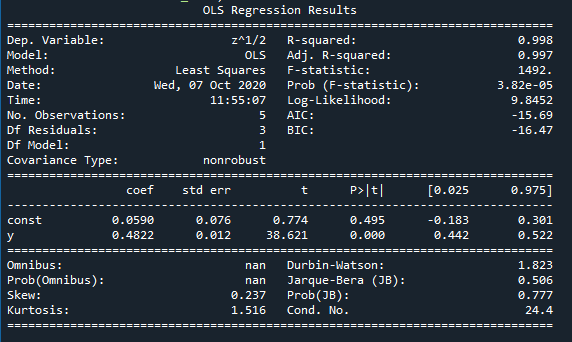
\includegraphics{2.2 6a.png}\\
where we find that our P value is much greater than $.05$. Therefore, we fail to 
reject the null hypothesis that the y-intercept is zero. Since our $R^2$ value is also
quite close to $1$, we say that the data is indeed proportional. Therefore, running our 
model again forcing the y-intercept to be zero: \\
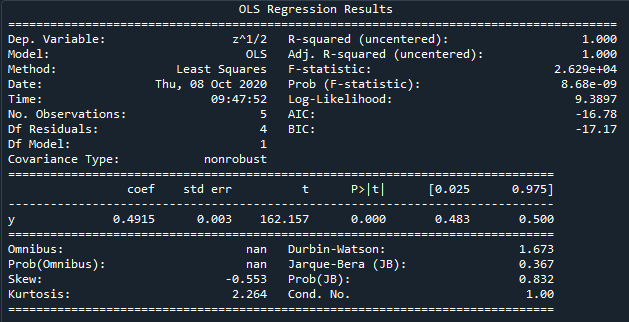
\includegraphics{2.2 6b.png}
We find from the model that our proportionality constant is $.4915$, therefore, our slope
$k = .4915$

\item  2.2 \#10
Using the data given and fitting an OLS regression: \\
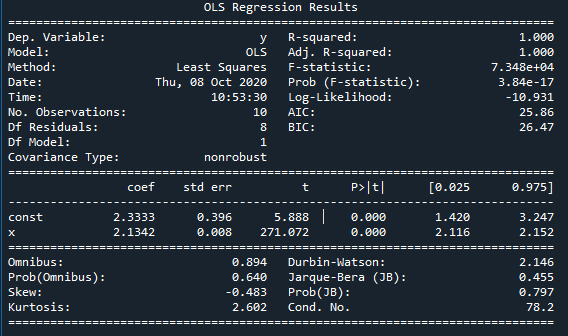
\includegraphics{2.2 10a.png}\\
we see that the p-value is less than $.05$ therefore, we can conclude that in this case, 
$y$ is not proportional to $x^2$. 

\item 2.3), \#2
Since we assume density is constant, we know weight is proportional to the volume: 
\begin{eqnarray*}
  W &=& kV\\
  W &=& k(L^3) \\
  \frac{W}{L^3} &=& k\\
  k &=& \frac{20}{3^3}\\
  k &=& \frac{20}{9}\\
  k &\approx& 2.2222
\end{eqnarray*}

Therefore, for a 100-lb flamingo, 
\begin{eqnarray*}
  100 &=& 2.2222V\\
  \frac{100}{2.2222} &=& V\\
  \frac{100}{2.2222} &=& L^3\\
  L &=& \sqrt[3]{\frac{100}{2.2222}}\\
  L &\approx& 3.5569
\end{eqnarray*}

Which shows that a 100-lb flamingo would have length $3.5569$ft. Since the leg height is 
also proportional to the length of the flamingo: 
\begin{eqnarray*}
  L_{height} &=& mL_{leg} \\
  3 &=& 2m \\
  \frac{3}{2} &=& m
\end{eqnarray*}

and using our new height: 
\begin{eqnarray*}
  3.5569 &=& \frac{3}{2}L_{leg}  \\
  3.5569 \frac{2}{3} &=& L_{leg} \\
  L_{leg} &\approx& 2.3713
\end{eqnarray*}

So we see height of the 100-lb flamingo is about $3.5569$ft and the leg height of the 
100-lb flamingo is $2.3713$ft. 
\end{enumerate}

\end{document}